\begin{figure}[h]
    \centering
    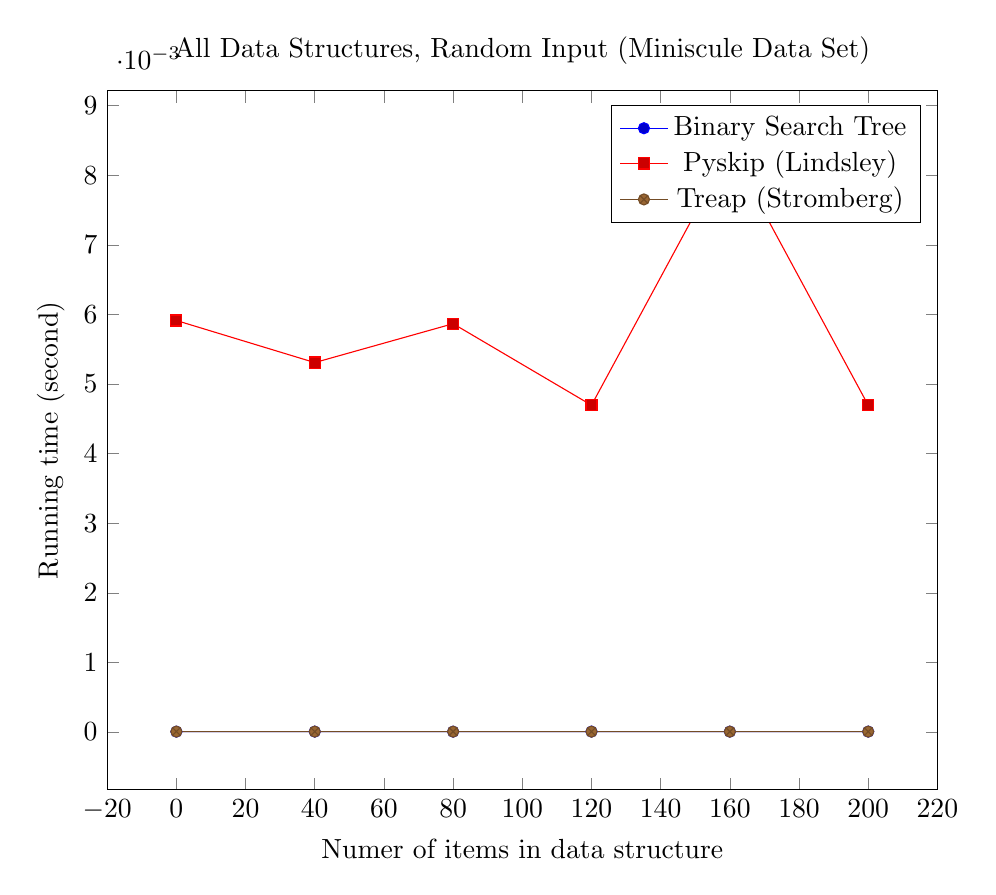
\begin{tikzpicture}
        \begin{axis}[
            xlabel={Numer of items in data structure},
            ylabel={Running time (second)},
            title={All Data Structures, Random Input (Miniscule Data Set)},
            width=\textwidth
        ]
		\addplot coordinates {
			(0, 4.638100185960781e-06)
			(40, 4.8790404553411545e-06)
			(80, 4.517630051292798e-06)
			(120, 5.360920994190721e-06)
			(160, 4.939275522719555e-06)
			(200, 5.029628123764951e-06)
		};
		\addplot coordinates {
			(0, 0.0059129753864455735)
			(40, 0.005308215310248254)
			(80, 0.005866925677456258)
			(120, 0.0046957752629637195)
			(160, 0.00837472235398642)
			(200, 0.004695112677222868)
		};
		\addplot coordinates {
			(0, 5.481391128858704e-06)
			(40, 5.391038527857717e-06)
			(80, 4.8489229217185684e-06)
			(120, 4.638100185960781e-06)
			(160, 4.96939305643096e-06)
			(200, 5.391038527857717e-06)
		};
        \legend{Binary Search Tree, Pyskip (Lindsley), Treap (Stromberg)}
        \end{axis}
    \end{tikzpicture}
    \caption{Average of 10 operations, benchmarked every 40, starting at 0.}
\end{figure}